\paragraph{}

Σε αυτό το κεφάλαιο καταπιανόμαστε με τα μοντέλα μηχανικής μάθησης που χρησιμοποιήσαμε για την μοντελοποίηση της επικοινωνίας, τις λεπτομέρειες που αφορούν τα εξαγόμενα χαρακτηριστικά από τις εφαρμογές, και τα benchmarks που χρησιμοποιήσαμε με σκοπό την εξαγωγή των σημείων που προορίζονται για την εκπαίδευση των μοντέλων επικοινωνίας.


\section{Μηχανική Μάθηση}
Όπως αναφέραμε πιο πάνω, σκοπός της δουλειάς μας είναι η πρόβλεψη του χρόνου επικοινωνίας μιας εφαρμογής με τεχνικές μηχανικής μάθησης και συγκεκριμένα, επιτηρούμενης μάθησης (supervised learning). Για την εκπαίδευση του μοντέλου, απαιτείται η χρήση κάποιων δειγμάτων, τα οποία σε όρους μηχανικής μάθησης αποτελούν το σύνολο εκπαίδευσης (training set). Κάθε ένα από αυτά τα δείγματα περιέχει ένα διάνυσμα χαρακτηριστικών (feature vector) και τη τιμή της μεταβλητής που το μοντέλο καλείται να προβλέψει. 
\paragraph{}
Η ακρίβεια του μοντέλου στηρίζεται σε πολλές παραμέτρους. Αρχικά, τα χαρακτηριστικά που επιλέγει κανείς πρέπει να αντικατοπτρίζουν τη συμπεριφορά της μεταβλητής. Ωστόσο, υπερβολικός αριθμός χαρακτηριστικών εισάγει μεγάλη πολυπλοκότητα στο μοντέλο, έτσι πρέπει να συμπεριλαμβάνουμε χαρακτηριστικά στο training set με φειδώ. Τέλος, συνίσταται το training set να περιλαμβάνει δείγματα για ένα μεγάλο εύρος των χαρακτηριστικών, σε αναλογία με τις περιπτώσεις που θέλουμε να προβλέψουμε.
\paragraph{}
Στην περίπτωση της εργασίας μας, τα χαρακτηριστικά του training set ήταν μετρικές εξαγόμενες με βάση τις παραμέτρους εκτέλεσης του MPI, την εφαρμογή, και τη θέση των διεργασιών στους πόρους του συστήματος, ενώ η μεταβλητή που το μοντέλο καλείται να προβλέψει είναι ο χρόνος επικοινωνίας. Αφού ο χρόνος παίρνει συνεχείς τιμές το πρόβλημα ανήκει στην κατηγορία της παλινδρόμησης (regression). Τέλος, σημειώνουμε ότι επιλέξαμε χαρακτηριστικά τα οποία μπορούν να εξαχθούν χωρίς την εκτέλεση της εφαρμογής. Σε άλλη περίπτωση η έννοια της πρόβλεψης δεν έχει νόημα. 

\subsection{Μέθοδοι για Regression}
\paragraph{}
Για την επίλυση προβλημάτων regression έχουν προταθεί πολλές μέθοδοι. Παραμετρικά μοντέλα, όπου τα χαρακτηριστικά πολλαπλασιασμένα με βάρη (παραμέτρους) σχηματίζουν μία συνάρτηση, γραμμική ή μη, είναι αρκετά συνήθη. Τέτοια μοντέλα απαιτούν τον ορισμό της μορφής της συνάρτησης από το χρήστη που πρέπει να έχει συναίσθηση του πως τα χαρακτηριστικά επηρεάζουν τη μεταβλητή, με τη μέθοδο να αναλαμβάνει τον υπολογισμό των παραμέτρων ικανοποιώντας κάποιο κριτήριο. Επιπρόσθετα, είναι ευάλωτα στην <<κατάρα της διαστασιμότητας>> με την πολυπλοκότητα του μοντέλου να αυξάνει εκθετικά με τον αριθμό των χαρακτηριστικών. Ωστόσο παρέχουν μία κλειστή συνάρτηση που συνδέει αναλυτικά την μεταβλητή με τα χαρακτηριστικά.
\paragraph{}
Από την άλλη μεριά μη παραμετρικά μοντέλα, όπως δέντρα αποφάσεων και μέθοδοι που συνδυάζουν τα αποτελέσματα τους(ensemble methods) κάνουν τη διαδικασία της εκπαίδευσης πολύ πιο αυτοματοποιημένη. Επιλέγουν ποια χαρακτηριστικά επηρεάζουν τη μεταβλητή περισσότερο, δεν απαιτούν καμιά κανονικοποίηση στις τιμές των χαρακτηριστικών ενώ καμία πληροφορία για το πως τα χαρακτηριστικά συσχετίζονται με τη μεταβλητή δεν πρέπει να δοθεί από το χρήστη. Επιπλέον, αφού τα περισσότερα χρησιμοποιούν δεντρικές δομές, δεν επηρεάζονται αρνητικά αν τα χαρακτηριστικά έχουν μη γραμμική σχέση με τη μεταβλητή.
\subsection{Μέθοδοι Ensemble}
\paragraph{}
Η μέθοδος που χρησιμοποιούμε ανήκει στην κατηγορία ensemble. Η βασική ιδέα είναι η σύνθεση προβλέψεων από απλές μεθόδους regression με σκοπό την αναπαράσταση από το μοντέλο περίπλοκων συναρτήσεων, μείωση της διασποράς των αποτελεσμάτων και περιορισμού της υπερ-προσαρμογής (overfitting) των μοντέλων στο training set. Στις περισσότερες περιπτώσεις, οι αλγόριθμοι βασίζονται σε απλά δέντρα αποφάσεων. Ανάλογα με τον τρόπο που συνθέτουν τα αποτελέσματά τους, οι αλγόριθμοι χωρίζονται σε δύο κατηγορίες: τις Bagging Μεθόδους, όπως τα  random forest και τα extremely randomized trees που προβλέπουν τη μεταβλητή με βάση το μέσο όρο των προβλέψεων των επιμέρους δέντρων και τις Boosting Μεθόδους, όπως την AdaBoost και την Gradient Boosting Regressor Tree όπου σε κάθε βήμα δημιουργούν νέους εκτιμητές που δίνουν έμφαση στα σημεία που τα προηγούμενα μοντέλα δεν υπολόγιζαν με αρκετή ακρίβεια. 

\subsection{Αλγόριθμος Gradient Boosting Regression Tree}
\paragraph{}
Στα πειράματα μας κάναμε εκτεταμένη χρήση του αλγορίθμου \textit{Gradient Boosting Regression Tree} (GBRT \cite{GBRT}), η υλοποίηση του οποίου παρέχεται στο \textit{scikit-learn} της \textit{Python} \cite{scikit}. Καθώς πρόκειται για Boosting μέθοδο, σε κάθε επανάληψη δημιουργείται ένας νέος εκτιμητής ο οποίος προσαρμόζεται στο ήδη υπάρχων μοντέλο με βάση την αρνητική βαθμίδα (gradient) μίας συνάρτησης υπολογισμού του σφάλματος. 
\paragraph{}
O GBRT μας δίνει τη δυνατότητα να ρυθμίσουμε αρκετές παραμέτρους με σκοπό την επίτευξη καλύτερων αποτελεσμάτων ανάλογα με τις ιδιαιτερότητες των δειγμάτων. Για την επίτευξή καλύτερων προβλέψεων εξετάσαμε σωρεία παραμέτρων. Συγκεκριμένα, οι παράμετροι που μας απασχόλησαν ήταν:
\begin{itemize}
\item[] \textbf{n\_estimator:} Ο αριθμός των δέντρων απόφασης που θα ενταχθούν επαναληπτικά στο τελικό δέντρο. Ταυτίζεται με τον αριθμό των επαναλήψεων.
\item[] \textbf{learning\_rate:} Ο ρυθμός μάθησης. Αφορά τον αντίκτυπο που έχει ένα νέο δέντρο στο ήδη υπάρχων.

\item[] \textbf{min\_samples\_split:} Ο ελάχιστος αριθμός δειγμάτων για να σπάσει ένας υπάρχων κόμβος σε δύο.

\item[] \textbf{min\_samples\_leaf:} Ο ελάχιστος αριθμός δειγμάτων για να θεωρηθεί ένας κόμβος, φύλλο.

\item[] \textbf{max\_depth:} Το μέγιστο βάθος που μπορεί να φτάσει το δέντρο.

\item[] \textbf{loss:} Η συνάρτηση υπολογισμού του σφάλματος. Δίνεται δυνατότητα επιλογής από μερικές προκαθορισμένες. 
\end{itemize}

\paragraph{}
Ωστόσο, οι μη παραμετρικές μέθοδοι, συμπεριλαμβανομένου και του αλγορίθμου GBRT, δεν μας παρέχουν με μία κλειστή αναλυτική μορφή για το πως προκύπτει ο χρόνος επικοινωνία. Παρόλα αυτά, με τη βοήθεια του scikit-learn, μπορέσαμε να εξάγουμε μία διαβάθμιση για τα χαρακτηριστικά με σκοπό να βγάλουμε συμπεράσματα σχετικά με το ποια επηρεάζουν περισσότερο το χρόνο επικοινωνίας. Η διαβάθμιση αυτή δεν είναι τελείως αντιπροσωπευτική αναφορικά με τα χαρακτηριστικά που επηρεάζουν την τελική πρόβλεψη. Για παράδειγμα, αν κάποιο χαρακτηριστικό βρίσκεται στα ψηλότερα επίπεδα του δέντρου απόφασης θα έχει αναπόφευκτα ψηλή θέση στη διαβάθμιση αλλά να απαιτείται και η συνδρομή άλλων χαρακτηριστικών στα χαμηλότερα επίπεδα για ακριβή πρόβλεψη.

\subsection{Επιλογή Χαρακτηριστικών}
\paragraph{}
Καθώς τα training set που εξετάζουμε περιέχουν σωρεία χαρακτηριστικών, σε μερικές περιπτώσεις κρίθηκε αναγκαία η χρήση μεθόδων επιλογής χαρακτηριστικών (feature selection) με σκοπό την απόρριψη μετρικών που δεν επηρεάζουν σημαντικά το χρόνο επικοινωνίας. Η μέθοδος που χρησιμοποιήσαμε στα πειράματα μας ήταν επιλογή χαρακτηριστικών μέσω της regression μεθόδου \textit{Support Vector Regressor (SVR)}. Συγκεκριμένα εκπαιδεύαμε ένα SVR μοντέλο με όλα τα δείγματα εκπαίδευσης. Μετέπειτα, με βάση τη διαβάθμιση της σημασίας(importance) που είχαμε στη διάθεση μας, αφαιρούσαμε από το αρχικό training set τα χαρακτηριστικά που είχαν μικρότερο importance από τον μέσο όρο των importances για όλα τα χαρακτηριστικά.

\subsection{Μέθοδοι εξαγωγής Communication Patterns}
\paragraph{}
Είχαμε στη διάθεσή μας αρκετές μεθόδους για την εξαγωγή των communication patterns. Η πιο εύκολη και ευθύγραμμη ήταν η προσθήκη συναρτήσεων στις εφαρμογές οι οποίες επιστρέφουν το communication pattern τους. Ωστόσο, αφού για τη ανάκτηση του communication pattern έπρεπε να έχει τελειώσει η εκτέλεση της εφαρμογής, δεν ήταν κατάλληλη για πρόβλεψη. Μία ανάλογη πρακτική, ήταν η επέκταση των εντολών αποστολής του \textit{OpenMPI} έτσι ώστε με κάθε κλήση των συναρτήσεων αποστολής μηνυμάτων να τυπώνουν τα αναγνωριστικά των διεργασιών που εμπλέκονται στην αποστολή και το μέγεθος των δεδομένων που αποστέλλονται. Η μεθοδολογία αυτή, πέραν του ότι είναι αρκετά περίπλοκη, εμφανίζει το ίδιο μειονέκτημα με την προηγούμενη και επίσης εγκαταλείφθηκε.

\paragraph{}
Τελικά, για κάθε εφαρμογή που μας απασχόλησε, είτε για σκοπούς benchmarking είτε για αξιολόγηση των μοντέλων επικοινωνίας, αναπτύξαμε σειριακές εκδόσεις που υπολόγιζαν το communication pattern τους. Τα ορίσματα τους περιελάμβαναν κάποιες από τις παραμέτρους εκτέλεσης των εφαρμογών, όπως τον αριθμό των MPI διεργασιών που έχουν άμεση επίδραση στις ανταλλαγές δεδομένων που λαμβάνουν χώρα, αλλά και ορίσματα συγκεκριμένα για κάθε εφαρμογή. Οι εκδόσεις αυτές δεν εκτελούσαν ούτε το υπολογιστικό κομμάτι, ούτε την επικοινωνία μεταξύ των διεργασιών. Έτσι δεν προσθέτουν πολυπλοκότητα στο κρίσιμο μονοπάτι της μεθοδολογίας μας. Τέλος, είναι ανεξάρτητες από το μηχάνημα και τη θέση των διεργασιών σε αυτό.

\paragraph{}
Το πιο σημαντικό πλεονέκτημα των σειριακών εκδόσεων, ήταν η δυνατότητα εξαγωγής των communication patterns πριν την εκτέλεση της εφαρμογής. Σαν αποτέλεσμα, σε κάποιο ρεαλιστικό σενάριο βελτιστοποίησης, μπορούμε να χρησιμοποιήσουμε τα μοντέλα μας για να πάρουμε τις προβλέψεις πριν την εκτέλεση της εφαρμογής, και με βάση τα αποτελέσματα να επιλέξουμε το configuration που μας παρέχει τα περισσότερα πλεονεκτήματα σχετικά με το μέγεθος των πόρων που θα χρησιμοποιήσουμε και το χρόνο επικοινωνίας που απαιτείται.

\section{Εξαγόμενες Μετρικές}
\paragraph{}
Κρίσιμο κομμάτι στη μεθοδολογία μας ήταν η εξαγωγή των χαρακτηριστικών από τις εφαρμογές. Σαν χαρακτηριστικά, εξάγαμε μετρικές με βάση τον αριθμό των ζητούμενων πόρων, το μοτίβο επικοινωνίας της κάθε εφαρμογής και τη θέση των διεργασιών στο μηχάνημα. 

\paragraph{}
Παρόλο που υπάρχουν κοινές μετρικές για Non-Blocking point-to-point και collective επικοινωνία πολλές διαφέρουν όπως και η διαδικασία για την εξαγωγή τους. Στις δύο επόμενες υποενότητες παραθέτουμε αναλυτικά τη διαδικασία που ακολουθήσαμε για τους δύο τύπους επικοινωνίας ξεχωριστά.
\subsection{Εξαγωγή Μετρικών Non-Blocking Επικοινωνίας}
\paragraph{}
Όσο αφορά τις μετρικές για την Non-Blocking point-to-point επικοινωνία, με βάση τα δεδομένα που απαιτούν για την εξαγωγή τους, τις χωρίσαμε σε τρεις κατηγορίες. Ο πρώτος τύπος μετρικών ήταν οι παράμετροι που δίνονται στο σύστημα εκτέλεσης του MPI πριν την εκτέλεση της εφαρμογής από το χρήστη. Η πληροφορία είναι απαραίτητη στη μεθοδολογία μας καθώς αποτελεί βάση για τις επόμενες μετρικές που εξάγαμε.
\paragraph{}
Ο δεύτερος τύπος, ήταν μετρικές εξαγόμενες από το προφίλ επικοινωνίας (com\-munication pattern) της κάθε εφαρμογής. Βασιζόμενοι σε αυτό υπολογίσαμε μετρικές στο επίπεδο της MPI διεργασίες. Οι μετρικές αυτές είναι ανεξάρτητες από το mapping των διεργασιών στους διαθέσιμους πόρους. Περιέχουν πληροφορίες για επικοινωνία που λαμβάνει χώρα από τη σκοπιά της διεργασίας-αποστολέας, αγνοώντας την απόσταση της από τη διεργάσία-παραλήπτης.
\paragraph{}
Παρόλα τα πλεονεκτήματα τους, οι προηγούμενες μετρικές αποτυγχάνουν να αποτυπώσουν τη διαφορά ανάμεσα στην επικοινωνία που λαμβάνει χώρα πάνω από το δίκτυο διασύνδεσης των NUMA κόμβων και την επικοινωνία εσωτερικά του κόμβου\footnote{Στα επόμενα βήματα θα αναφερόμαστε στην επικοινωνία μεταξύ των NUMA κόμβων σαν internode και στην επικοινωνία εσωτερικά των κόμβων σαν intranode, αφού στην κλίμακα των μηχανημάτων που μας αφορούν οι κόμβοι είναι τα NUMA islands.}. Σαν αποτέλεσμα, για επόμενο τύπο μετρικών επιλέξαμε μετρικές που βασίζονται στην κατανομή των διεργασιών στους πόρους του συστήματος και στο communication pattern της εφαρμογής. Έτσι εξάγαμε μετρικές στο επίπεδο του κόμβου πετυχαίνοντας το στόχο μας, για διάκριση της επικοινωνίας σε intranode και internode. 

\paragraph{}
Είναι σημαντικό να αναφέρουμε ότι, για να εφαρμόσουμε τη μεθοδολογία μας, ήταν απαραίτητη η γνώση της απεικόνισης των MPI διεργασιών στους πόρους του μηχανήματος. Έτσι σε όλα τα πειράματα μας η θέση των διεργασιών στους πόρους δινόταν ρητώς στο σύστημα εκτέλεσης του MPI. Ισοδύναμα, αν το περιβάλλον εκτέλεσης ανάθετε τις διεργασίες στους πόρους με συγκεκριμένη πολιτική (blocked,round-robin etc), μπορούσαμε να υπολογίσουμε ευθύγραμμα την απεικόνιση πριν την εκτέλεση της εφαρμογής. Η ρητή επιλογή της απεικόνισης κρίθηκε πιο βολική, αφού μας έδινε τη δυνατότητα να πάρουμε δείγματα εκπαίδευσης για σωρεία διαφορετικών mappings που είναι άμεσα συσχετισμένα με τον τρίτο τύπο μετρικών. Παρόλα αυτά, δεν πρόκειται για δεσμευτική επιλογή. Η μοναδική προϋπόθεση είναι η γνώση της απεικόνισης πριν τη εκτέλεση της εφαρμογής.
\paragraph{}
Επιπλέον, όλες οι μετρικές είναι υπολογισμένες με βάση τα δεδομένα που αποστέλλονται αγνοώντας αν κάποια διεργασία λαμβάνει πολύ περισσότερα δεδομένα από ότι αποστέλλει με ότι αυτό συνεπάγεται για την επικοινωνία. Εντούτοις, σε περιπτώσεις στις οποίες διεργασίες αποστέλλουν πολλά δεδομένα χωρίς να λαμβάνουν ανάλογο αριθμό, κοινή πρακτική είναι η χρήση άλλων μεθόδων αποστολής δεδομένων και όχι point-to-point επικοινωνίας.  

\paragraph{}
Παρακάτω θα αναφερθούμε αναλυτικά σε όλες τις μετρικές που εξάγαμε για κάθε τύπο.
\paragraph{Μετρικές με βάση τις παραμέτρους εκτέλεσης του MPI}
\begin{itemize}
\item \textbf{Κόμβοι} \textit{(Νodes-N)} : Ο αριθμός των κόμβων στους οποίους εκτελείται η εφαρμογή. 
\item \textbf{Διεργασίες ανά Κόμβο} \textit{(ProcessesPerNode-PPN)} : Ο αριθμός των MPI διεργασιών ανά κόμβο. Επηρεάζει τον όγκο της επικοινωνίας εσωτερικά του κόμβου, ανάλογα με το communication pattern της εφαρμογής.
\item \textbf{Σύνολο MPI διεργασιών} \textit{(Processes-P)} : Ο συνολικός αριθμός των MPI διεργασιών που ζητά ο χρήστης.
\end{itemize}

\paragraph{Μετρικές με βάση το μοτίβο επικοινωνίας της εφαρμογής\\} 
Οι μετρικές αυτές είναι υπολογισμένες ανά διεργασία. Στο τελικό training set περιέχεται η ελάχιστη, μέση και μέγιστη τιμή τους. 
\begin{itemize}
\item \textbf{Μέγεθος Μηνυμάτων ανά διεργασία} \textit{(Size-S)} :  Το μέγεθος των μηνυμάτων που αποστέλλονται από τις διεργασίες. Για μεγάλα μηνύματα το πρωτόκολλο επικοινωνίας μπορεί να αλλάξει.
\item \textbf{Αριθμός Μηνυμάτων ανά διεργασία} \textit{(Messages-M)} : Το άθροισμα των μηνυμάτων που αποστέλλονται από κάθε διεργασία. Ανάλογα με τον αριθμό των μηνυμάτων, μηνύματα ίσως σειριοποιούνται ή  συνενώνονται. 
\item \textbf{Όγκος Δεδομένων ανά διεργασία} \textit{ (ProcessTraffic-PT) } : Το άθροισμα των μηνυμάτων που αποστέλνονται ανά διεργασία. Ο όγκος των δεδομένων ανά διεργασία μπορεί να εντοπίσει φαινόμενα συμφόρησης. 
\end{itemize}

\paragraph{Μετρικές με βάση την κατανομή των διεργασιών στο μηχάνημα και το μοτίβο επικοινωνίας\\}
Για όσες μετρικές από αυτές είναι υπολογισμένες ανά κόμβο, στο training set περιλαμβάνεται η ελάχιστη, μέση και μέγιστη τιμή τους.
\begin{itemize}
\item \textbf{Εσωτερικός Όγκος Δεδομένων ανά κόμβο} \textit{(IntraΝodeΤraffic-NT)} : Αφορά τον όγκο των δεδομένων που ανταλλάσσουν διεργασίες που βρίσκονται στον ίδιο κόμβο. Μπορεί να αντικατοπτρίσει περιπτώσεις συμφόρησης στο διάδρομο δεδομένων εντός του κόμβου. 
\item \textbf{Εσωτερικός Αριθμός Μηνυμάτων ανά κόμβο} \textit{(IntraΝodeΙnjection-NI)} : Ο αριθμός των μηνυμάτων ανάμεσα σε διεργασίες που βρίσκονται στον ίδιο κόμβο.
\item \textbf{Συνολικός Όγκος Δεδομένων εσωτερικά των κόμβων} \textit{(Int\-raVolume-V)} : Όλος ο όγκος των δεδομένων ανάμεσα σε διεργασίες που βρίσκονται στον ίδιο κόμβο. Πρόκειται ουσιαστικά για το άθροισμα όλων των \textit{IntraNodeTraffics}.
\item \textbf{Συνολικός αριθμός μηνυμάτων εσωτερικά των κόμβων} \textit{(Int\-raInjection-VI)} : Το πλήθος όλων των μηνυμάτων που αποστέλλονται εσωτερικά των κόμβων. 
\item \textbf{Εξωτερικός Όγκος Δεδομένων ανά κόμβο} \textit{(InterNodeTraffic-INT)} : Ο όγκος των δεδομένων ανάμεσα σε διεργασίες που βρίσκονται σε διαφορετικούς κόμβους. Μπορεί να αντικατοπτρίσει περιπτώσεις συμφόρησης στο δίκτυο διασύνδεσης των νησιών NUMA. 
\item \textbf{Εξωτερικός Αριθμός Μηνυμάτων ανά κόμβο} \textit{(InterΝodeΙnjection-INI)} : Ο αριθμός των μηνυμάτων που αποστέλλονται σε διεργασίες που βρίσκονται σε άλλο κόμβο.
\item \textbf{Συνολικός Όγκος Δεδομένων εξωτερικά των κόμβων} \textit{(Int\-erVolume-IV)} : Όλος ο όγκος των δεδομένων ανάμεσα σε διεργασίες που βρίσκονται σε διαφορετικούς κόμβους. Πρόκειται ουσιαστικά για το άθροισμα όλων των \textit{InterNodeTraffics}.
\item \textbf{Συνολικός αριθμός μηνυμάτων εξωτερικά των κόμβων} \textit{(Int\-erInjection-IVI)} : Το πλήθος όλων των μηνυμάτων ανάμεσα σε διεργασίες που βρίσκονται σε διαφορετικούς κόμβους. 
\end{itemize}

\subsection{Εξαγωγή Μετρικών Collective Επικοινωνίας}
\paragraph{}
Η επιλογή και η εξαγωγή των μετρικών για την Collective επικοινωνία ήταν πολύ πιο περίπλοκη διαδικασία σε σχέση με την point-to-point. Οι αλγόριθμοι που χρησιμοποιούνται διαφέρουν από υλοποίηση σε υλοποίηση και αλλάζουν συνεχώς. Συνήθως, τα collectives $scatter,gather$ και $reduce$ βασίζονται σε point-to-point υλοποιήσεις, το $broadcast$ σε ένα δεντρικό αλγόριθμο και τα $allreduce,allgather$ και $alltoall$ σε συνδυασμό των παραπάνω. Η μεγαλύτερη πρόκληση ήταν να κρατήσουμε τη μεθοδολογία μας ανεξάρτητη της υλοποίησης του κάθε collective. Επομένως, θα ήταν πολύ πιο φορητή και θα μπορούσε να εφαρμοστεί και σε άλλες υλοποιήσεις των collectives. Αυτό σήμαινε ότι δεν θα είχαμε στη διάθεση μας το ακριβές communication pattern για κάθε εφαρμογή. Έτσι, για την μοντελοποίηση της επικοινωνίας στηριχτήκαμε σε ένα αφηρημένο communication pattern που φτιάξαμε, ανάλογα με τον κάθε τύπο collective.
\paragraph{}
Θα προσπαθήσουμε να εξηγήσουμε τη λογική μας μέσω ενός παραδείγματος. Ας πάρουμε για παράδειγμα το communication pattern που δίνει η μοντελοποίηση για το collective allgather. Tο συγκεκριμένο collective μαζεύει δεδομένα από όλες τις διεργασίες και τα επιστρέφει σε όλες. Έστω ότι έχουμε ένα allgather με buffer εισόδου μεγέθους $S$ bytes και $N$ MPI διεργασίες. Υποθέτουμε ότι όλοι οι buffers πρέπει να μαζευτούν σε κάποια διεργασία και μετέπειτα να αποσταλούν στις υπόλοιπες. Έτσι όλες οι διεργασίες αποστέλλουν ένα μήνυμα μεγέθους $S$ σε κάποια διεργασία "ρίζα",  η οποία με τη σειρά της αποστέλλει μηνύματα μεγέθους $N\times S$ σε όλες τις άλλες. Θα συμβολίζουμε αυτό το communication pattern με $N - 1 - N$, αφού σε πρώτο στάδιο $N$ διεργασίες αποστέλλουν δεδομένα σε 1 και σε επόμενο, 1 σε $N$. Ωστόσο αυτός ο συμβολισμός δεν περιέχει όλη την πληροφορία του communication pattern αφού δεν περιλαμβάνει το μέγεθος των μηνυμάτων. Για είμαστε πλήρης, θα χρησιμοποιήσουμε και ένα δεύτερο συμβολισμό, που θα περιέχει το μέγεθος των μηνυμάτων που ανταλλάσσονται σε κάθε στάδιο. Έτσι, για το allgather έχουμε το συμβολισμό $S-(N\times S)$ αφού μηνύματα $S$ μεγέθους αποστέλλονται στο πρώτο στάδιο και μηνύματα $N\times S$ στο δεύτερο. Στον Πίνακα \ref{table:coll} φαίνεται πώς μοντελοποιήσαμε κάθε collective που μας απασχόλησε.
\begin{table}[t]
\centering
\caption{Communication Pattern για κάθε collective}
\label{table:coll}
\begin{tabular}{l|c|c}
\textbf{Collective} & \textbf{Μηνύματα} & \textbf{Μέγεθος Μηνυμάτων} \\ \hline
scatter    & 1-N      & S                 \\
gather     & N-1      & S                 \\
reduce     & N-1      & S                 \\
broadcast  & 1-N      & S                 \\
allreduce  & N-1-N    & S-S               \\
allgather  & N-1-N    & S-(N$\times$S)           \\
alltoall   & N-N      & S                
\end{tabular}
\end{table}

\paragraph{}
Αφού πλέον είχαμε στη διάθεση μας τα communication patterns, 	μπορούσαμε να προχωρήσουμε στην επιλογή των μετρικών. Αναλογικά με την point-to-point επικοινωνία χωρίζουμε τις μετρικές σε τρεις κατηγορίες: την πρώτη, που ήταν η ίδια με την point-to-point επικοινωνία και αφορούσε τις παραμέτρους που δίνονται στο σύστημα εκτέλεσης του MPI, τη δεύτερη που περιείχε τις μετρικές που εξάγονται από το communication pattern και την τρίτη με τις μετρικές βασίζονταν στο communication pattern και στο mapping των διεργασιών στο μηχάνημα. 

\paragraph{}
Σε αντίθεση με τις μετρικές της point-to-point επικοινωνίας, στις μετρικές της collective επικοινωνίας έχουμε μετρικές που αφορούν τα δεδομένα που αποστέλλονται αλλά και τα δεδομένα που λαμβάνονται καθώς η επικοινωνία δεν είναι συμμετρική. Παρακάτω παραθέτουμε τις μετρικές για κάθε τύπο αναλυτικά. 
\paragraph{Μετρικές με βάση τις παραμέτρους εκτέλεσης του MPI}
\begin{itemize}
\item \textbf{Κόμβοι} \textit{(Νodes-N)} : Ο αριθμός των κόμβων στους οποίους εκτελείται η εφαρμογή. 
\item \textbf{Διεργασίες ανά Κόμβο} \textit{(ProcessesPerNode-PPN)} : Ο αριθμός των MPI διεργασιών ανά κόμβο. Επηρεάζει τον όγκο της επικοινωνίας εσωτερικά του κόμβου, ανάλογα με το communication pattern της εφαρμογής.
\item \textbf{Σύνολο MPI διεργασιών} \textit{(Processes-P)} : Ο συνολικός αριθμός των MPI διεργασιών.
\end{itemize}

\paragraph{Μετρικές με βάση το μοτίβο επικοινωνίας της εφαρμογής\\} 
Οι μετρικές αυτές είναι υπολογισμένες ανά διεργασία. Στο τελικό training set περιέχεται η ελάχιστη, μέση και μέγιστη τιμή τους. 
\begin{itemize}
\item \textbf{Μέγεθος Μηνυμάτων ανά διεργασία} \textit{(Size-S)} :  Το μήκος των μηνυμάτων που αποστέλλονται από τις διεργασίες.
\item \textbf{Πλήθος Μηνυμάτων ανά διεργασία} \textit{(Messages-M)} : Το πλήθος των μηνυμάτων που αποστέλλονται από κάθε διεργασία.
\item \textbf{Εισερχόμενος Όγκος Δεδομένων ανά διεργασία} \textit{ (IncomingProcess\-Traffic-IPT) } : Το άθροισμα των μεγεθών των  μηνυμάτων που λαμβάνονται ανά διεργασία. 
\item \textbf{Εξερχόμενος Όγκος Δεδομένων ανά διεργασία} \textit{ (OutgoingProcess\-Traffic-ΟPT) } : Το άθροισμα των μεγεθών μηνυμάτων που αποστέλλονται ανά διεργασία.
\end{itemize}

\paragraph{Μετρικές με βάση την κατανομή των διεργασιών στο μηχάνημα και το μοτίβο επικοινωνίας\\}
Για όσες μετρικές από αυτές είναι υπολογισμένες ανά κόμβο, στο training set περιλαμβάνεται η ελάχιστη, μέση και μέγιστη τιμή τους.
\begin{itemize}
\item \textbf{Εσωτερικός Όγκος Δεδομένων ανά κόμβο} \textit{(Intra\-ΝodeΤraffic-NT)} : Αφορά τον όγκο των δεδομένων που ανταλλάσσουν διεργασίες που βρίσκονται στον ίδιο κόμβο. 
\item \textbf{Εσωτερικός Αριθμός Μηνυμάτων ανά κόμβο} \textit{(Intra\-ΝodeΙnjection-NI)} : Ο αριθμός των μηνυμάτων ανάμεσα σε διεργασίες που βρίσκονται στον ίδιο κόμβο.
\item \textbf{Συνολικός Όγκος Δεδομένων εσωτερικά των κόμβων} \textit{(Intra\-Volume-V)} : Όλος ο όγκος των δεδομένων ανάμεσα σε διεργασίες που βρίσκονται στον ίδιο κόμβο. 
\item \textbf{Συνολικός αριθμός μηνυμάτων εσωτερικά των κόμβων} \textit{(Intra\-Injection-VI)} : Το άθροισμα όλων των μηνυμάτων εσωτερικά των κόμβων. 
\item \textbf{Εξωτερικός Όγκος Εξερχόμενων Δεδομένων ανά κόμβο} \textit{(Inter\-NodeOutgoingTraffic-INOT)} : Ο όγκος των εξερχόμενων δεδομένων με προορισμό διεργασίες σε άλλο κόμβο. 
\item \textbf{Εξωτερικός Όγκος Εισερχόμενων Δεδομένων ανά κόμβο} \textit{(Inter\-NodeIncomingTraffic-INIT)} : Ο όγκος των εισερχόμενων δεδομένων με πηγή διεργασίες σε άλλο κόμβο.
\item \textbf{Εξωτερικός Αριθμός Εξερχόμενων Μηνυμάτων  ανά κόμβο} \textit{(Inter\-ΝodeOutgoingΙnjection-INOI)} : Το πλήθος των εξερχόμενων μηνυμάτων με προορισμό διεργασίες που βρίσκονται σε διαφορετικό κόμβο.
\item \textbf{Εξωτερικός Αριθμός Εισερχόμενων Μηνυμάτων  ανά κόμβο} \textit{(Inter\-ΝodeOutgoingΙnjection-INΙI)} : Το πλήθος των εισερχόμενων μηνυμάτων με πηγή διεργασίες σε άλλο κόμβο.
\item \textbf{Συνολικός Όγκος Εξερχόμενων Δεδομένων εξωτερικά των κόμβων} \textit{(Int\-erOutgoingVolume-IVO))} : Όλος ο όγκος των δεδομένων που αποστέλλονται προς διεργασίες που βρίσκονται σε διαφορετικούς κόμβους. 
\item \textbf{Συνολικός Αριθμός  Εξερχόμενων Μηνυμάτων εξωτερικά των κόμβων} \textit{(Int\-erInjection-IVOI)} : Το άθροισμα όλων των μηνυμάτων που αποστέλλονται με αποδέκτη εξωτερικά του κόμβου.
\item \textbf{Συνολικός Όγκος Δεδομένων εξωτερικά των κόμβων} \textit{(Int\-erVolume-IVI)} : Όλος ο όγκος των δεδομένων ανάμεσα σε διεργασίες που βρίσκονται σε διαφορετικούς κόμβους. Πρόκειται ουσιαστικά για το άθροισμα όλων των \textit{InterNodeTraffics}.
\item \textbf{Συνολικός αριθμός μηνυμάτων εξωτερικά των κόμβων} \textit{(Int\-erInjection-IVII)} : Το πλήθος όλων των μηνυμάτων εξωτερικά των κόμβων. 
\end{itemize}
\paragraph{}
\section{Benchmarking}
Όπως αναφέραμε πιο πάνω, αναπόσπαστο κομμάτι της μεθοδολογίας μας είναι η εξαγωγή δεδομένων μέσω benchmarks, τα οποία  χρησιμοποιήσουμε για την εκπαίδευση των μοντέλων επικοινωνίας. Επιλέξαμε benchmarks των οποίων η φάση επικοινωνίας θυμίζει επικοινωνία εφαρμογών, ενώ ταυτόχρονα μας δίνουν τη δυνατότητα ορισμού διαφόρων παραμέτρων με σκοπό την εξαγωγή ενός ευρύ χώρου μετρικών.

\subsection{p2p\_SRR}
\paragraph{}
Αρχικά θα αναφερθούμε στο benchmark p2p\_SRR (point-to-point symmetric with random ratio). Πρόκειται για ένα benchmark βασισμένο στο WICON benchmark \cite{WICON}, όπου τυχαία ζευγάρια κόμβων, με μία διεργασία να τρέχει στον καθένα, ανταλλάσσουν δεδομένα ταυτόχρονα σε μία ping-pong διαδικασία. Ωστόσο, στο p2p\_SRR μας δίνεται η δυνατότητα να τοποθετήσουμε περισσότερες από μία διεργασίες στον κάθε κόμβο. Επιπλέον, για να συμπεριλάβει στους χρόνους την επιρροή πολλών μηνυμάτων, κάθε διεργασία επικοινωνεί με τυχαίες M διεργασίες. Έτσι, καταλήγουμε σε ένα communication pattern στο οποίο κάθε διεργασία στέλνει M μηνύματα σε Μ τυχαίες διεργασίες και αντίστοιχα λαμβάνει απάντηση. Αυτό, σε NUMA αρχιτεκτονική οδηγεί σε ένα communication pattern όπου η αναλογία της internode και intranode επικοινωνίας είναι τυχαία.

\paragraph{}
Κάθε ανταλλαγή μηνυμάτων εκτελείται μερικές εκατοντάδες φορές και κάθε διεργασία μετρά τον τοπικό χρόνο που δαπάνησε για κάθε επανάληψη. Οφείλουμε να αναφέρουμε ότι, πριν την έναρξη κάθε επανάληψης οι διεργασίες συγχρονίζονται για να αποφύγουμε τη μέτρηση χρόνου αναμονής σαν χρόνο επικοινωνίας.  Αφού κάθε διεργασία ταξινομήσει τους χρόνους, ορίζει σαν τοπικό χρόνο επικοινωνίας  κάποιο ποσοστημόριο (quantile) των επαναλήψεων δικής μας επιλογής. Μετέπειτα, μέσω του collective reduce, η εφαρμογή επιστρέφει το μέγιστο χρόνο ανάμεσα από τους τοπικούς. Με αυτή τη τιμή εκπαιδεύσαμε και τα μοντέλα επικοινωνίας στα επόμενα στάδια. Παρόλο που είχαμε την ευχέρεια να επιλέξουμε οποιοδήποτε quantile επιλέξαμε το τρίτο  για να αντισταθμίσουμε αύξηση στο χρόνο επικοινωνίας από φαινόμενα που αγνοούσαμε (cache effects, os noise κ.α.). 
\paragraph{}
Επιπλέον, το benchmark, μας επέτρεπε να ορίσουμε δύο παραμέτρους: τον αριθμό των μηνυμάτων(\textit{M}), μέσω μίας παραμέτρου εισόδου και το μέγεθος του μηνύματος. με μικρές αλλαγές στον πηγαίο κώδικα. Ακόμη, μπορούσαμε να ελέγξουμε τον αριθμό των διεργασιών ανά κόμβο(\textit{PPN}) και τον αριθμό των κόμβων(\textit{N}) μέσω του συστήματος εκτέλεσης του MPI. Τελικά, είχαμε την ευχέρεια να διατρέξουμε τέσσερις παραμέτρους που είχαν άμεση εξάρτηση με όλες τις μετρικές, με αποτέλεσμα ένα training set μεγάλου μεγέθους και αρκετά διαφοροποιημένων σημείων. Το εύρος της κάθε παραμέτρου δίνεται στον Πίνακα \ref{table:NBp2p}.

\begin{table}[h]
\centering
\footnotesize
\caption{Ο χώρος παραμέτρων για το benchmark \textit{p2p\_SRR}}
\label{table:NBp2p}
\begin{tabular}{c|cc}
\multirow{2}{*}{Παράμετρος} & \multicolumn{2}{c}{Αρχιτεκτονική} \\ 
                            & UMA             & NUMA            \\ \hline \hline
N                           & 1               & 2-4             \\
PPN                         & 2-8             & 1-8             \\
Size                        & 1B-16MiB        & 1B-16MiB        \\
Messages                    & 1-8             & 1-8             \\ \hline
\#samples                   & 800             & 4000           
\end{tabular}
\end{table}

\paragraph{}
Παρόλα τα πλεονεκτήματα του, το \textit{p2p\_SRR} υλοποιεί μόνο ανταλλαγές μηνυμάτων ίσου μεγέθους. Τέτοιου τύπου communication patterns καλούνται κανονικά (regular).Σαν αποτέλεσμα, η ελάχιστη, μέση και μέγιστη τιμή που χρησιμοποιούμε από διάφορες μετρικές για χαρακτηριστικά να μην διαφέρουν.  Έτσι τα μοντέλα επικοινωνίας που εκπαιδεύονται με βάση το p2p\_SRR αποτυγχάνουν να διακρίνουν τη διαφορά μεταξύ τους. 

\subsection{p2p\_AS}
Για να αντιμετωπίσουμε το παραπάνω πρόβλημα χρησιμοποιήσαμε δημιουργήσαμε το benchmark p2p\_AS (point-to-point asymmetric sparse)  βασιζόμενοι στο μοτίβο επικοινωνίας της παράλληλης έκδοσης του αλγορίθμου \textit{Sparce Matrix Vector Multiplication} (SpMV) \cite{CG}. Πρόκειται για ένα αλγόριθμο που υλοποιεί παράλληλα τον πολλαπλασιασμό ενός αραιού πίνακα Α με ένα διάνυσμα.

\paragraph{}
Η ιδιαιτερότητα του communication pattern του \textit{p2p\_AS} είναι ότι έχει άμεση εξάρτηση από τη δομή και το μέγεθος του πίνακα $A$ με αποτέλεσμα για αρκετούς πίνακες να είναι ακανόνιστο (irregular). Σκοπός μας δεν ήταν να χρησιμοποιήσουμε ένα training set με δείγματα μόνο από irregular communication patterns αλλά να εμπλουτίσουμε το ήδη υπάρχων training set από regular δείγματα με irregular. Έτσι, εισάγουμε στο training set την πληροφορία για να μπορεί να αντιληφθεί το μοντέλο το διαφορετικό αντίκτυπο των μετρικών, χωρίς να θυσιάζουμε τα ποικίλα σημεία που εξάγουμε από το \textit{p2p\_SRR}. Κατά την εκτέλεση, είχαμε και πάλι τη δυνατότητα, να ελέγχουμε το PPN και τον αριθμό των κόμβων με τον ίδιο τρόπο όπως στο \textit{p2p\_SRR}. Ωστόσο δεν είχαμε άμεσο έλεγχο στον αριθμό των μηνυμάτων και στο μέγεθός τους, το οποίο πλέον διέφερε για κάθε MPI διεργασία. Οι δύο αυτές μετρικές ήταν παράγωγα του πίνακα εισόδου, $A$. Έτσι αρκεστήκαμε να διατρέχουμε τις παραμέτρους N και PPN και μία λίστα πινάκων εισόδου του \textit{SpVM}, βλ. Πίνακες \ref{table:CG},\ref{table:CG_matrices} και Σχήμα \ref{fig:CG}. Σαν αποτέλεσμα, τα δείγματα που εξάγαμε ήταν πολύ λιγότερα σε σχέση με το πλήθος των \textit{p2p\_SRR}. Τέλος, αφού ο αλγόριθμος είναι επαναληπτικός, ο τελικός χρόνος επιλέγετε όπως στο \textit{p2p\_SRR} ενώ πριν την έναρξη της επικοινωνίας εισάγεται \textit{Barrier} για την αποφυγή μέτρησης άεργου χρόνου σαν χρόνο επικοινωνίας. 

\begin{table}
\centering
\footnotesize
\caption{Ο χώρος παραμέτρων για το benchmark \textit{p2p\_AS}}
\label{table:CG}
\begin{tabular}{c|cc}
\multirow{2}{*}{Παράμετρος} & \multicolumn{2}{c}{Αρχιτεκτονική} \\ 
                            & UMA             & NUMA            \\ \hline \hline
N                           & 1               & 2-4             \\
PPN                         & 2-8             & 1-8             \\
Size                        & 96B-2MiB($\sim$)     & 8B-4MiB($\sim$)        \\
Messages                    & 0-7             & 0-31             \\ \hline
\#samples                   & 55              & 335           
\end{tabular}
\end{table}

\begin{figure}[H]
    \centering
    \begin{subfigure}[b]{0.3\textwidth}
        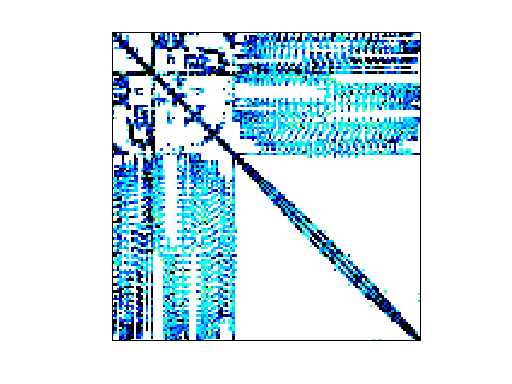
\includegraphics[width=\textwidth]{./images/CG/audi.png}
        \caption{audikw\_1}
    \end{subfigure}
    \quad 
    \begin{subfigure}[b]{0.3\textwidth}
        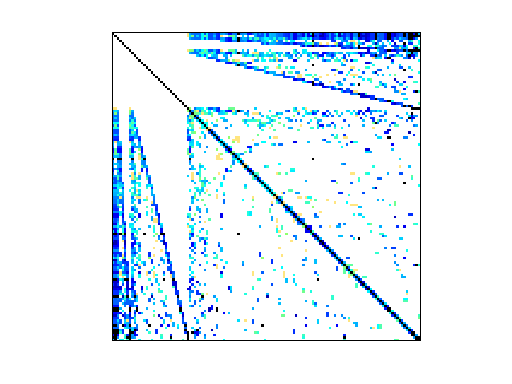
\includegraphics[width=\textwidth]{./images/CG/helm2d03.png}
        \caption{helm2d03}
    \end{subfigure}
    \quad 
	\begin{subfigure}[b]{0.3\textwidth}
        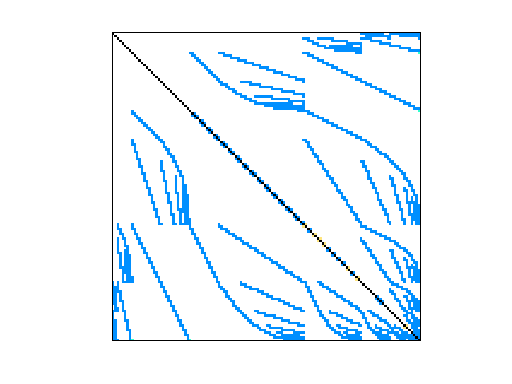
\includegraphics[width=\textwidth]{./images/CG/parabolic_fem.png}
        \caption{parabolic\_fem}
    \end{subfigure}
    \quad 
    \begin{subfigure}[b]{0.3\textwidth}
        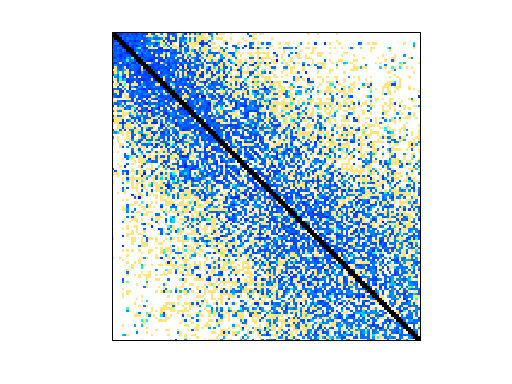
\includegraphics[width=\textwidth]{./images/CG/nd24k.png}
        \caption{nd24k}
    \end{subfigure}
    \quad 
    \begin{subfigure}[b]{0.3\textwidth}
        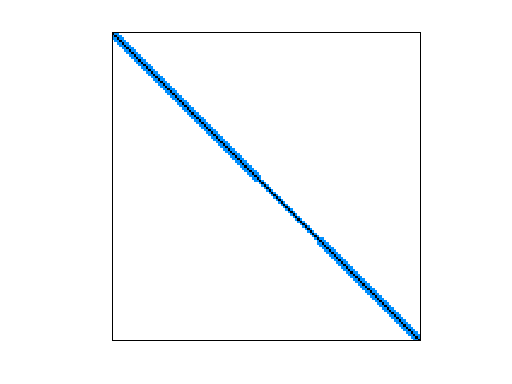
\includegraphics[width=\textwidth]{./images/CG/bone010.png}
        \caption{bone010}
    \end{subfigure}
    \quad 
    \begin{subfigure}[b]{0.3\textwidth}
        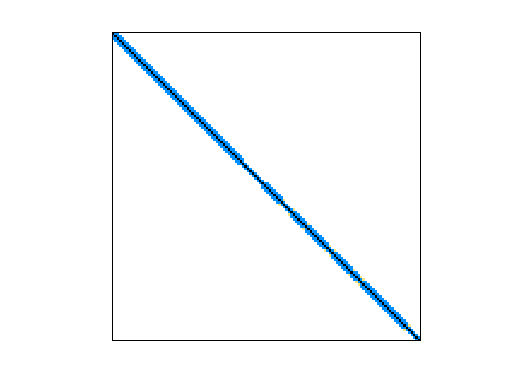
\includegraphics[width=\textwidth]{./images/CG/boneS10.png}
        \caption{boneS10}
    \end{subfigure}
    \quad 
    \begin{subfigure}[b]{0.3\textwidth}
        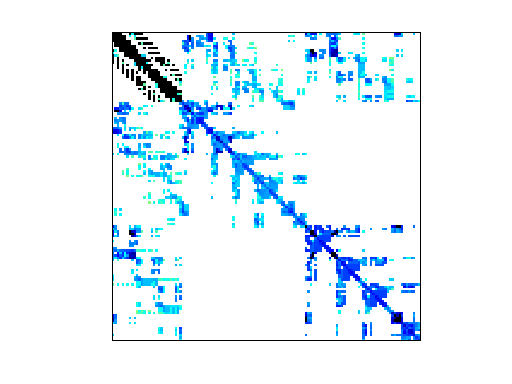
\includegraphics[width=\textwidth]{./images/CG/thread.png}
        \caption{thread}
    \end{subfigure}
    \quad 
    \begin{subfigure}[b]{0.3\textwidth}
        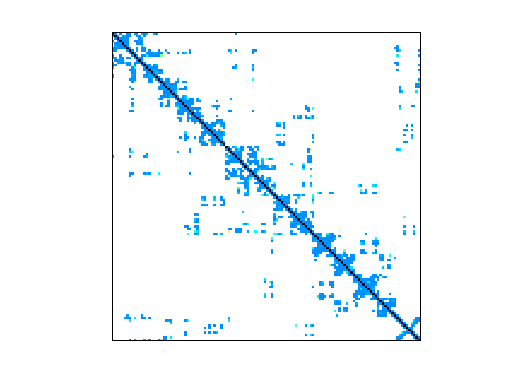
\includegraphics[width=\textwidth]{./images/CG/pdb1HYS.png}
        \caption{pdbHYS}
    \end{subfigure}
    \quad 
    \begin{subfigure}[b]{0.3\textwidth}
        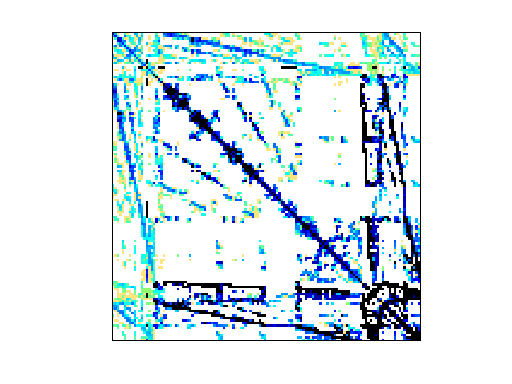
\includegraphics[width=\textwidth]{./images/CG/crankseg_1.png}
        \caption{crankseg\_1}
    \end{subfigure}
    \quad 
    \begin{subfigure}[b]{0.3\textwidth}
        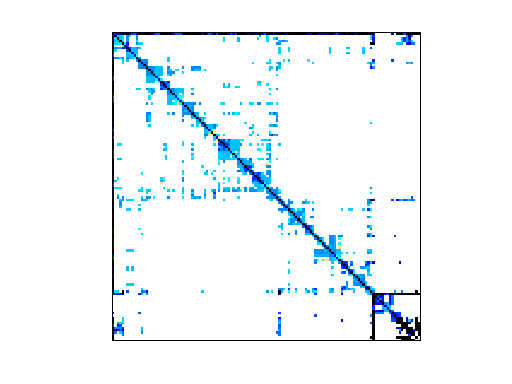
\includegraphics[width=\textwidth]{./images/CG/rajat30.png}
        \caption{rajat30}
    \end{subfigure}
    \quad 
    \begin{subfigure}[b]{0.3\textwidth}
        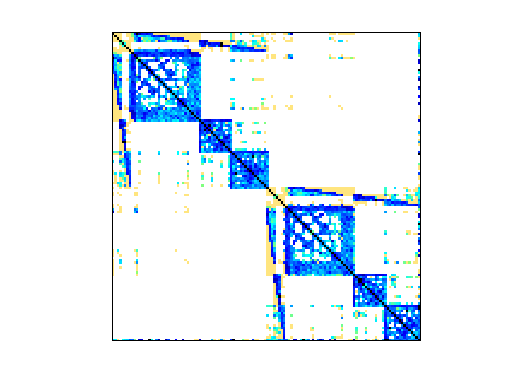
\includegraphics[width=\textwidth]{./images/CG/inline_1}
        \caption{inline\_1}
    \end{subfigure}
    \quad 
    \begin{subfigure}[b]{0.3\textwidth}
        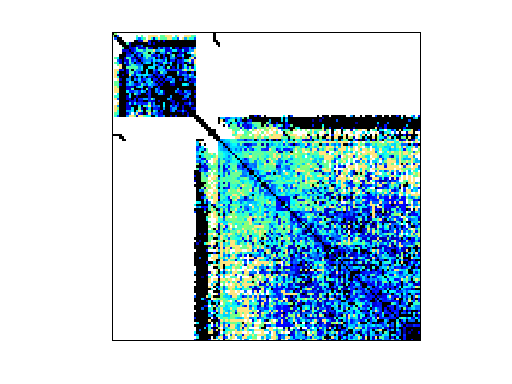
\includegraphics[width=\textwidth]{./images/CG/ldoor.png}
        \caption{ldoor}
    \end{subfigure}
    \quad 
    \begin{subfigure}[b]{0.3\textwidth}
        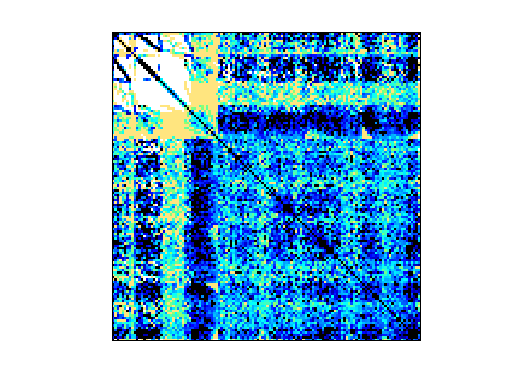
\includegraphics[width=\textwidth]{./images/CG/F1.png}
        \caption{F1}
    \end{subfigure}
    \quad 
    \begin{subfigure}[b]{0.3\textwidth}
        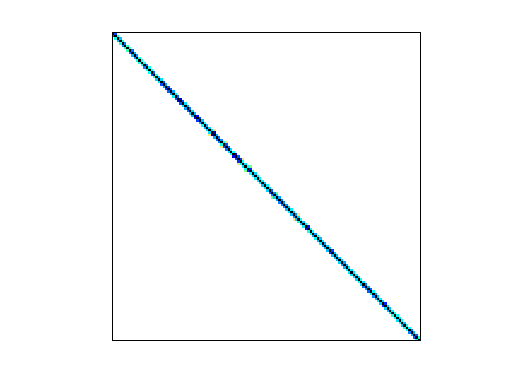
\includegraphics[width=\textwidth]{./images/CG/af_shell9.png}
        \caption{af\_shell9}
    \end{subfigure}
    \quad 
    \begin{subfigure}[b]{0.3\textwidth}
        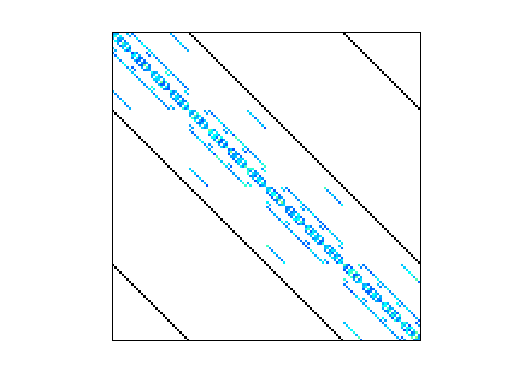
\includegraphics[width=\textwidth]{./images/CG/conf5_0-4x4-26.png}
        \caption{conf5\_0-4x4-26}
    \end{subfigure}
    \quad 
    \begin{subfigure}[b]{0.3\textwidth}
        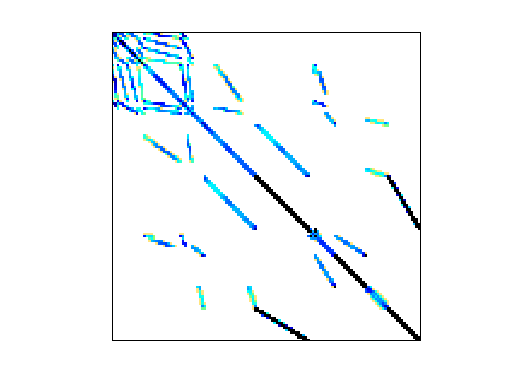
\includegraphics[width=\textwidth]{./images/CG/HV15R.png}
        \caption{HV15R}
    \end{subfigure}
    \quad 
    \caption{Πίνακες εισόδου για το benchmark \textit{p2p\_AS}}
    \label{fig:CG}
\end{figure}

\begin{table}[h]
\centering
\caption{Χαρακτηριστικά πινάκων εισόδου για το benchmark \textit{p2p\_AS}}
\label{table:CG_matrices}
\begin{tabular}{c|c|c}
$Name$ & $Size(\times 10^3)$ & $Non\ Zero\ Values (\times 10^6)$ \\ \hline \hline
audikw\_1 & 943.7 & 77.3 \\
helm2d03 & 392.3 & 2.7 \\
parabolic\_fem & 525.8 & 3.7 \\
nd24k & 72.0 &  28.7 \\
bone010 & 986.7 & 47.9 \\
boneS10 & 914.9 & 40.9 \\
thread & 29.7 & 4.4 \\
pdb1HYS & 36.4 & 4.3 \\
crankseg\_1 & 52.8 & 10.6 \\
rajat30 & 644.0 & 6.2 \\
inline\_1 & 503.7 & 36.8 \\
ldoor & 952.2 & 42.5 \\
F1 & 343.8 & 26.8 \\
af\_shell9 & 504.9 & 17.6\\
conf5\_0-4x4-26 & 3.1 & 0.1 \\
HV15R & 2017.2 & 283.1 \\    
\end{tabular}
\end{table}

\subsection{NB\_SFR}
\paragraph{}
Η ανάπτυξη του benchmark \textit{p2p\_SFR} (point-to-point symmetric with fixed ratio) έγινε με αφορμή την αδυναμία του \textit{p2p\_SRR} να καθορίσει εκ των προτέρων την αναλογία internode και intranode επικοινωνίας. Όπως αναφέραμε, στο benchmark p2p\_SRR κάθε διεργασία επιλέγει τυχαία τη διεργασία που θα ανταλλάξει δεδομένα για κάθε μήνυμα που θα αποστείλει. Ωστόσο, οι τοπικές διεργασίες είναι πολύ λιγότερες από αυτές που βρίσκονται σε άλλο κομβο με αποτέλεσμα, να υπάρχει μεγαλύτερη πιθανότητα να επιλεγούν. Στα περισσότερα σημεία προερχόμενα από p2p\_SRR, η intranode επικοινωνία αποτελούσε περίπου το 25\% της συνολικής επικοινωνίας ανάλογα πάντα και με τον αριθμό των διεργασιών ανά κόμβο. Για την αποφυγή του φαινομένου αυτού, στο benchmark \textit{p2p\_SFR} έχουμε τη δυνατότητα να ορίσουμε εκ των προτέρων την αναλογία intranode και internode επικοινωνίας  επιλέγοντας πόσες διεργασίες ανά κομβό θα επικοινωνούν τοπικά. Το μεγαλύτερο μειονέκτημα του είναι ότι απαιτεί γνώση της αρχιτεκτονικής του μηχανήματος, σε αντίθεση με το \textit{p2p\_SRR}. Ο χώρος παραμέτρων του είναι ο ίδιος με το \textit{p2p\_SRR} με επιπλέον την προσθήκη μίας παραμέτρου εισόδου, $INP$, που ορίζει των αριθμό των διεργασιών που επικοινωνούν εσωτερικά του κόμβου που εκτελούνται, βλ. Πίνακα \ref{table:NBINP}. Τέλος, το benchmark δεν είναι εφαρμόσιμο σε UMA αρχιτεκτονικές αφού δεν λαμβάνει χώρα internode επικοινωνία.

\begin{table}[h]
\centering
\caption{Ο χώρος παραμέτρων για το benchmark \textit{p2p\_SFR}}
\label{table:NBINP}
\begin{tabular}{c|c}
\multirow{1}{*}{Παράμετρος} & \multicolumn{1}{c}{Αρχιτεκτονική} \\ 
                                        & NUMA            \\ \hline \hline
N                                         & 2-4             \\
PPN                                      & 1-8             \\
Size                               & 1B-16MiB        \\
Messages                                & 1-8             \\ 
INP						     & 2/4/6/8(<PPN) \\ \hline
\#samples                               & 8800 \\  \
\end{tabular}
\end{table}



\subsection{Collective}
\paragraph{}
Επιπρόσθετα από τα benchmarks που αφορούσαν την point-to-point επικοινωνία, χρειαστήκαμε και benchmark για την εξαγωγή δειγμάτων εκπαίδευσης για την collective επικοινωνία. Δημιουργήσαμε ξεχωριστά benchmarks για κάθε collective που εξετάσαμε βασισμένοι στα \textit{OSU Micro-Benchmarks}\footnote{http://mvapich.cse.ohio-state.edu/benchmarks/} και τα benchmarks που παρέχει για την collective επικοινωνία του MPI. H αρχική έκδοση των benchmarks, εκτελεί τον τύπο του collective που αφορά, για μερικές εκατοντάδες επαναλήψεις και ένα εύρος από μήκος δεδομένων εισόδου. Για κάθε μήκος επιστρέφει τον μέσο όρο του χρόνου επικοινωνίας από όλες τις επαναλήψεις. Στη δική μας έκδοση, ακολουθούμε το πρότυπο των δύο προηγούμενων benchmarks, όπου ο χρόνος επιλέγεται σαν το μέγιστο κάποιου quantile των τοπικών χρόνων επαναλήψεων και εισάγεται Barrier πριν την έναρξη της επικοινωνίας σε κάθε επανάληψη. Επιλέχθηκε ξανά το τρίτο quantile για τους ίδιους λόγους με το \textit{p2p\_SRR}. O χώρος παραμέτρων δίνεται στον Πίνακα \ref{table:collectives}. Σε αντίθεση με τη point-to-point επικοινωνία, δεν ελέγχαμε το μήκος των μηνυμάτων που ανταλλάσσονται αλλά το μέγεθος των δεδομένων εισόδου \footnote{Στην point-to-point επικοινωνία το μήκος δεδομένων εισόδου ισούται με το μήκος των μηνυμάτων. Κάτι τέτοιο δεν ισχύει σε όλα τα collectives, βλ. Allgather}. Το μήκος των μηνυμάτων εξαρτάται από την υλοποίηση και τον τύπο του collective. 

\begin{table}[h]
\centering
\caption{Ο χώρος παραμέτρων για τα benchmarks \textit{Collective}}
\label{table:collectives}
\begin{tabular}{c|cc}
\multirow{2}{*}{Παράμετρος} & \multicolumn{2}{c}{Αρχιτεκτονική} \\ 
                            & UMA             & NUMA            \\ \hline \hline
N                           & 1               & 2-4             \\
PPN                         & 2-8             & 1-8             \\
Input Size                 & 4B-1MiB     & 4B-1MiB        \\ \hline
\textbf{\#samples}                   & 656              & 2460 
\end{tabular}
\end{table}




